\documentclass[english]{article}
\usepackage[utf8]{inputenc}
\usepackage{acronym}
\usepackage{amsmath}
\usepackage{graphicx}
\usepackage{longtable}
\usepackage{textgreek}
\usepackage{listings}
\usepackage{hyperref}
\usepackage[export]{adjustbox}
\lstset{
    escapeinside={(*}{*)}
}
\usepackage{todonotes}
\usepackage[english]{babel}
\usepackage{setspace}
\hyphenation{li-mitations}

\graphicspath{{figures/}}

\title{
	\vspace{-3cm}
	\center{
		
\includegraphics[width=0.5\textwidth, center]{unipi_logo.jpg}
		\linebreak
		\center{\large{DIPARTIMENTO DI INGEGNERIA\\DELL'INFORMAZIONE}}\\
		\vspace{10mm}
		{\large\textbf{\singlespacing A framework for validation of bio-inspired exploration algorithm in multi-robot scenarios }}
		\vspace{5mm}\\
		\large{MSc. Computer Engineering}
		\vspace{3mm}
		\normalsize{
			\begin{flushleft}
				\textit{Supervisors:}
				\linebreak
				\linebreak
				Prof.Cinzia BERNARDESCHI\\
				Prof. Andrea DOMENICI\\
				Dott. Maurizio PALMIERI
			\end{flushleft}
			\begin{flushright}
				\textit{Candidate:}
				\linebreak
				\linebreak
				Pietro CIRAVOLO
			\end{flushright}
		}
		\author{}
		\date{}
		\vspace{20mm}
		\normalsize{\author{\textit{Academic Year: 2019/2020}}}
	}
}


\begin{document}

\maketitle
\thispagestyle{empty}

\clearpage\null\thispagestyle{empty}\newpage

\section*{Acknowledgements}
\thispagestyle{empty}
I wish to express my deepest gratitude to the professor Cinzia Bernardeschi, for giving me the opportunity to be introduced in the scope of Digital Twin approach for modeling and simulation of Cyber-Physical Systems. Together with her, I want to thank Maurizio Palmieri and the professors Adriano Fagiolini and Andrea Domenici, that gave me their complete availability, supporting me during the whole work period. The great experience and competence of them, guided me, allowing a productive and particularly positive working climate.\\
\\Then I want to thank Gabriele Scoma, old friend and colleague with whom I share all the difficulties but also the satisfactions of this educational path.\\
\\A special person that must be thanked is my girlfriend and colleague Joana, that never had doubts on my possibilities to reach objectives, every time I doubted of myself. \\ 
\\Finally, a special regard must be given to my father Attilio, my mother Letizia, my sister Sara and my brother Luca. Is impossible to quantify the importance that each of them has in my life. Their constant support and sacrifices enabled me to overcome difficulties and reach the completion of this challenging and interesting degree course.   

\clearpage\null\thispagestyle{empty}\newpage

\setcounter{page}{1}


\tableofcontents

\clearpage

\section*{Acronyms List}

\begin{acronym}

\end{acronym}

\clearpage

\listoffigures

\clearpage

\listoftables

\clearpage

\section*{Abstract}
\thispagestyle{empty}            

\clearpage

\section{Introduction}
\label{Introduction to the thesis work}      

\clearpage

\section{Related work}
\label{Related work}

\section{Background}
\label{Background}

\subsection{The bio-inspired exploration algorithms}
\label{The bio-inspired exploration algorithms}

\subsection{The Unicycle Point to Point control algorithm}
\label{The Unicycle Point to Point control algorithm}

\subsection{FMI standard}
\label{FMU-FMI standard}

\subsection{Design Space Exploration}
\label{Design Space Exploration}

\subsection{INTO-CPS project}
\label{INTO-CPS project}

\subsection{Development tools}
\label{Development tools and simulation environment}

\subsubsection{INTO-CPS Application}
\label{INTO-CPS Application}

\subsubsection{PVSio-Web}
\label{PVSio-Web}

\subsection{Programming languages and libraries}
\label{Programming languages and libraries}

\section{Co-simulation architecture}
\label{Co-simulation architecture}
In this section is described the co-simulation architecture which has been considered suitable for the aim of our project. The chosen architecture is able to offer a good solution for a class of algorithms, similar to that discussed in this thesis. The Functional Mock-up Units (FMU) which make up the co-simulation architecture are:
\begin{itemize}
	\item Environment FMU
	\item Body\_Block FMU
	\item Controller FMU
\end{itemize}
\noindent Section \ref{Overall architecture of the Cyber-Physical System} describes the overall co-simulation architecture.\\
\\ Section \ref{The Environment FMU} provides a complete description of the modeled Environment FMU.\\
\\Section \ref{The Controller FMU} provides a complete description of the modeled Controller FMU.\\
\\The Body\_Block FMU provides the kinematics of robots involved in the experiments. In our work, we have considered suitable to use the Body\_Block FMU provided in the INTO-CPS example project \url{https://github.com/into-cps/case-study_line_follower_robot}.  

\subsection{Overall architecture of the Cyber-Physical System}
\label{Overall architecture of the Cyber-Physical System}
The exploration algorithms like that we want to model~\cite{AlgorithmPaper}, use "stigmergy" to share local knowledge of the environment information, necessary for the robot to be able to establish its next objective. From a logical point of view, the environment should only provides some information to the robots. The robots should be able to use this information and execute some calculations to find the next way point. Unfortunately, the complexity of the calculations to be performed is very high. An Arduino robot may not be able to perform them. For this reason, our choice is to move, the execution of the exploration algorithm, entirely inside the Environment FMU, obtaining a central module with coordination role.\\
\\Each robot is composed by two modules: the Boby\_Block FMU and the Controller FMU.\\
\\In the following figure is showed the whole co-simulation architecture:

\begin{figure} [h]
	\centering
	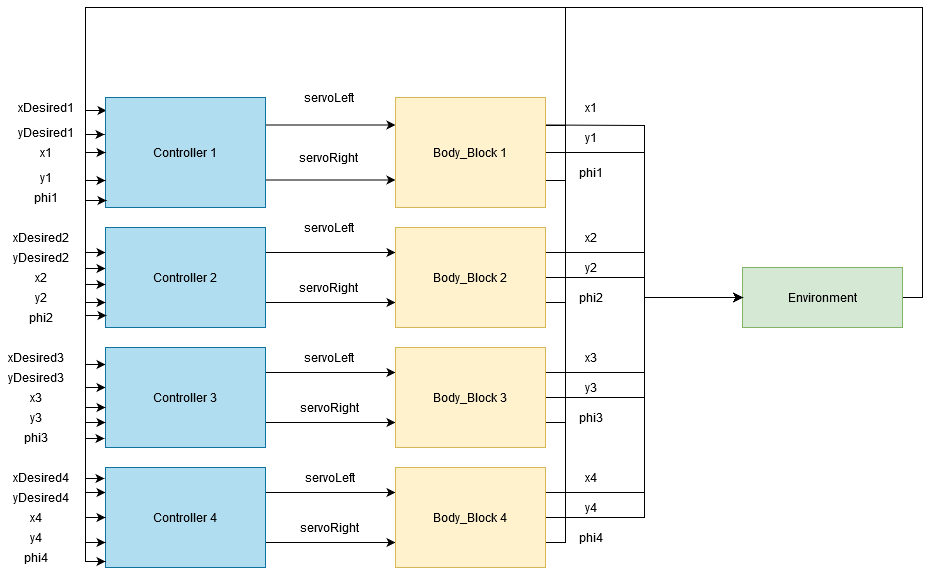
\includegraphics[width=0.7\linewidth]{figures/architecture.png}
	\caption{Co-simulation architecture}
	\label{fig:architecture}
\end{figure}

\subsection{The Environment FMU}
\label{The Environment FMU}
The Environment FMU is the module that represents the physical spatial environment where, all the robots that are involved in an exploration algorithm, are allowed to move. 
\\During the modeling of the Environment FMU, we put a very high attention on the scenario customization aspect. The goal is to obtain a module that can be configured with different scenarios. Some important customization parameters are listed below:
\begin{itemize}
	\item Map side length (only square)
	\item Number of robots that can communicate with the environment
	\item Number of obstacles
	\item Coordinates of the robots
	\item Coordinates of the obstacles 
\end{itemize}
\noindent It is important to give information about some limits of this customization:
\begin{itemize}
	\item The maximum number of robots is fixed
	\item The maximum number of obstacles is fixed
\end{itemize}
\noindent The reason of this limits is that the Environment FMU has no possibility to dynamically creates variables for the communication with an infinite number of robots, or to the management of an indefinite number of obstacles. So, chosen a reasonable quantity for both, a certain number of variables has been created.\\
\\Another important information to give, is that the Environment FMU has been implemented in a preliminary version where the robots are abstracts. In this way we have the possibility to perform a preliminary co-simulation to test the correct execution of the exploration algorithm. Then, a second version has been implemented, which includes the input/output variables needed to allow the right communication with the other modules. In order to allow the co-simulation using the preliminary Environment version, an input variable without a specific role " has been created to allow the connection with a second FMU named "ShowOutput". This FMU simply connect its output variable to that of the Environment, allowing the co-simulation. Then, in order to perform DSE analysis, the output variables of the Environment FMU interested in the ranking phase, has been connected to two input variable with the same name in ShowOutput FMU. This is not probably an elegant solution, but has been considered suited for the aim of the next work steps.  
\\In the two table below are listed all the input/output variables and the parameters that can be used to configure the environment scenario and the exploration algorithm: 

\begin{longtable}{|c|c|c|c|}
	\hline
	\textbf{Name} & 
	\textbf{Type} & 
	\textbf{Scope} &
	\textbf{Description} \\ \hline
	\endfirsthead
	%
	\endhead
	%
	dummy & Integer & Input & \\ \hline
	eP & Real & Output & give the map exploration percentage\\ \hline
	sTime & Real & Output & give the simulation time length\\ \hline
	nRobots & Integer & Local & number of robots\\ \hline
	mapSize & Integer & Local & map side length \\ \hline 
	nObstacles & Integer & Local & number of obstacles in the map \\ \hline
	stepCount & Integer & Local & number of passed co-simulation steps \\ \hline
	step\_size & Double & Local & time length of a co-simulation step \\ \hline
	s\_range & Integer & Local & range of the sporing in cells \\ \hline
	a1 & Double & Local & see section\ref{The bio-inspired exploration algorithms} \\ \hline
	a2 & Double & Local & see section\ref{The bio-inspired exploration algorithms} \\ \hline
	ertu\_perc & Double & Local & see section \ref{The bio-inspired exploration algorithms} \\ \hline
	eta & Double & Local & see section\ref{The bio-inspired exploration algorithms} \\ \hline
	max\_ph & Double & Local & see section\ref{The bio-inspired exploration algorithms} \\ \hline
	phi & Double & Local & see section\ref{The bio-inspired exploration algorithms} \\ \hline
	lambda & Double & Local & see section\ref{The bio-inspired exploration algorithms} \\ \hline
	ox\_1 & Integer & Local & x coordinate of the obstacle 1 \\ \hline
	ox\_2 & Integer & Local & x coordinate of the obstacle 2 \\ \hline
	ox\_3 & Integer & Local & x coordinate of the obstacle 3 \\ \hline
	ox\_4 & Integer & Local & x coordinate of the obstacle 4 \\ \hline
	ox\_5 & Integer & Local & x coordinate of the obstacle 5 \\ \hline
	ox\_6 & Integer & Local & x coordinate of the obstacle 6 \\ \hline
	ox\_7 & Integer & Local & x coordinate of the obstacle 7 \\ \hline
	ox\_8 & Integer & Local & x coordinate of the obstacle 8 \\ \hline
	ox\_9 & Integer & Local & x coordinate of the obstacle 9 \\ \hline
	ox\_10 & Integer & Local & x coordinate of the obstacle 10 \\ \hline
	oy\_1 & Integer & Local & y coordinate of the obstacle 1 \\ \hline
	oy\_2 & Integer & Local & y coordinate of the obstacle 2 \\ \hline
	oy\_3 & Integer & Local & y coordinate of the obstacle 3 \\ \hline
	oy\_4 & Integer & Local & y coordinate of the obstacle 4 \\ \hline
	oy\_5 & Integer & Local & y coordinate of the obstacle 5 \\ \hline
	oy\_6 & Integer & Local & y coordinate of the obstacle 6 \\ \hline
	oy\_7 & Integer & Local & y coordinate of the obstacle 7 \\ \hline
	oy\_8 & Integer & Local & y coordinate of the obstacle 8 \\ \hline
	oy\_9 & Integer & Local & y coordinate of the obstacle 9 \\ \hline
	oy\_10 & Integer & Local & y coordinate of the obstacle 10 \\ \hline
	x\_1 & Double & Local & x coordinate of the robot 1 \\ \hline
	x\_2 & Double & Local & x coordinate of the robot 2 \\ \hline
	x\_3 & Double & Local & x coordinate of the robot 3 \\ \hline
	x\_4 & Double & Local & x coordinate of the robot 4 \\ \hline
	y\_1 & Double & Local & y coordinate of the robot 1 \\ \hline
	y\_2 & Double & Local & y coordinate of the robot 2 \\ \hline
	y\_3 & Double & Local & y coordinate of the robot 3 \\ \hline
	y\_4 & Double & Local & y coordinate of the robot 4 \\ \hline
	port & Integer & Local & the port of the web socket connection \\ \hline
	\caption{Variables and parameters of preliminary version of the Environment FMU}
	\label{tab:label1}
\end{longtable}

\begin{longtable}{|c|c|c|c|}
	\hline
	\textbf{Name} & 
	\textbf{Type} & 
	\textbf{Scope} &
	\textbf{Description} \\ \hline
	\endfirsthead
	%
	\endhead
	%
	x\_1 & Double & Input & take the x coordinate robot 1 \\ \hline
	x\_2 & Double & Input & take the x coordinate robot 2 \\ \hline
	x\_3 & Double & Input & take the x coordinate robot 3 \\ \hline
	x\_4 & Double & Input & take the x coordinate robot 4 \\ \hline
	y\_1 & Double & Input & take the y coordinate robot 1 \\ \hline
	y\_2 & Double & Input & take the y coordinate robot 2 \\ \hline
	y\_3 & Double & Input & take the y coordinate robot 3 \\ \hline
	y\_4 & Double & Input & take the y coordinate robot 4 \\ \hline
	onDestination1Input & Integer & Input & used for synchronization \\ \hline
	onDestination2Input & Integer & Input & used for synchronization \\ \hline
	onDestination3Input & Integer & Input & used for synchronization \\ \hline
	onDestination4Input & Integer & Input & used for synchronization \\ \hline
	onDestinationOutput & Integer & Output & used for synchronization \\ \hline
	xDesired1 & Double & Output & x of robot 1 destination\\ \hline
	xDesired2 & Double & Output & x of robot 2 destination\\ \hline
	xDesired3 & Double & Output & x of robot 3 destination\\ \hline
	xDesired4 & Double & Output & x of robot 4 destination\\ \hline
	yDesired1 & Double & Output & y of robot 1 destination\\ \hline
	yDesired2 & Double & Output & y of robot 2 destination\\ \hline
	yDesired3 & Double & Output & y of robot 3 destination\\ \hline
	yDesired4 & Double & Output & y of robot 4 destination\\ \hline
	eP & Real & Output & give the map exploration percentage\\ \hline
	sTime & Real & Output & give the simulation time length\\ \hline
	nRobots & Integer & Local & number of robots\\ \hline
	mapSize & Integer & Local & map side length \\ \hline 
	nObstacles & Integer & Local & number of obstacles in the map \\ \hline
	stepCount & Integer & Local & number of passed co-simulation steps \\ \hline
	step\_size & Double & Local & time length of a co-simulation step \\ \hline
	s\_range & Integer & Local & range of the sporing in cells \\ \hline
	a1 & Double & Local & see section\ref{The bio-inspired exploration algorithms} \\ \hline
	a2 & Double & Local & see section\ref{The bio-inspired exploration algorithms} \\ \hline
	ertu\_perc & Double & Local & see section \ref{The bio-inspired exploration algorithms} \\ \hline
	eta & Double & Local & see section\ref{The bio-inspired exploration algorithms} \\ \hline
	max\_ph & Double & Local & see section\ref{The bio-inspired exploration algorithms} \\ \hline
	phi & Double & Local & see section\ref{The bio-inspired exploration algorithms} \\ \hline
	lambda & Double & Local & see section\ref{The bio-inspired exploration algorithms} \\ \hline
	ox\_1 & Integer & Local & x coordinate obstacle 1 \\ \hline
	ox\_2 & Integer & Local & x coordinate obstacle 2 \\ \hline
	ox\_3 & Integer & Local & x coordinate obstacle 3 \\ \hline
	ox\_4 & Integer & Local & x coordinate obstacle 4 \\ \hline
	ox\_5 & Integer & Local & x coordinate obstacle 5 \\ \hline
	ox\_6 & Integer & Local & x coordinate obstacle 6 \\ \hline
	ox\_7 & Integer & Local & x coordinate obstacle 7 \\ \hline
	ox\_8 & Integer & Local & x coordinate obstacle 8 \\ \hline
	ox\_9 & Integer & Local & x coordinate obstacle 9 \\ \hline
	ox\_10 & Integer & Local & x coordinate obstacle 10 \\ \hline
	oy\_1 & Integer & Local & y coordinate obstacle 1 \\ \hline
	oy\_2 & Integer & Local & y coordinate obstacle 2 \\ \hline
	oy\_3 & Integer & Local & y coordinate obstacle 3 \\ \hline
	oy\_4 & Integer & Local & y coordinate obstacle 4 \\ \hline
	oy\_5 & Integer & Local & y coordinate obstacle 5 \\ \hline
	oy\_6 & Integer & Local & y coordinate obstacle 6 \\ \hline
	oy\_7 & Integer & Local & y coordinate obstacle 7 \\ \hline
	oy\_8 & Integer & Local & y coordinate obstacle 8 \\ \hline
	oy\_9 & Integer & Local & y coordinate obstacle 9 \\ \hline
	oy\_10 & Integer & Local & y coordinate obstacle 10 \\ \hline
	lx\_1 & Double & Local & x coordinate robot 1 \\ \hline
	lx\_2 & Double & Local & x coordinate robot 2 \\ \hline
	lx\_3 & Double & Local & x coordinate robot 3 \\ \hline
	lx\_4 & Double & Local & x coordinate robot 4 \\ \hline
	ly\_1 & Double & Local & y coordinate robot 1 \\ \hline
	ly\_2 & Double & Local & y coordinate robot 2 \\ \hline
	ly\_3 & Double & Local & y coordinate robot 3 \\ \hline
	ly\_4 & Double & Local & y coordinate robot 4 \\ \hline
	port & Integer & Local & the port of the web socket connection \\ \hline
	\caption{Variables and parameters of definitive version of the Environment FMU}
	\label{tab:label2}
\end{longtable}  

\noindent There are some significant differences between the two lists. The coordinates of the robots become input variables that take a value directly from the robots FMUs. Nevertheless, during the first step the environment must be able to know the robots initial positions that are given by a set of local variables. The variables "onDestination" are used to allow the correct synchronization between the Environment and robots FMUs. In fact, the Environment wait for all the robots reached the objective, before to compute the new way points. When the Environment compute these positions, it needs to communicate this information to the robots controllers.\\
\\In the following paragraphs are analyzed the methods of definitive version of the Environment FMU. It constitutes the more complete version and involves all the code of the preliminary version. All the methods are defined in the file Environment.h and are implemented in the file Environment.c. 
Below there is the implementation of the method "setEnvironment":

\lstset{language=C++,
	basicstyle=\ttfamily,
	keywordstyle=\color{blue}\ttfamily,
	stringstyle=\color{red}\ttfamily,
	commentstyle=\color{gray}\ttfamily,
	breaklines=true
}
\begin{lstlisting}
/**
* Set the initial environment 
*/
void setEnvironment(State* st) {

 int32_t i,j;
 //Variables used to compute the exploration percentage
 nCells = st->mapSize*st->mapSize; //Total number of cells
 vCells = 0; //Total number of visited cells

 //Assignment of the initial robots coordinates
 st->x_1 = st->lx_1;
 st->x_2 = st->lx_2;
 st->x_3 = st->lx_3;
 st->x_4 = st->lx_4;
 st->y_1 = st->ly_1;
 st->y_2 = st->ly_2;
 st->y_3 = st->ly_3;
 st->y_4 = st->ly_4;
 st->xDesired1 = st->lx_1;
 st->xDesired2 = st->lx_2;
 st->xDesired3 = st->lx_3;
 st->xDesired4 = st->lx_4;
 st->yDesired1 = st->ly_1;
 st->yDesired2 = st->ly_2;
 st->yDesired3 = st->ly_3;
 st->yDesired4 = st->ly_4;

 map = (Cell**)malloc(st->mapSize*sizeof(Cell*));
 occupiedCells = (Cell**)malloc(st->nRobots*sizeof(Cell*));
 for(i = 0; i < st->mapSize; ++i)
  map[i] = (Cell*)malloc(st->mapSize*sizeof(Cell));

 x = (float64_t*)malloc(4*sizeof(float64_t));
 y = (float64_t*)malloc(4*sizeof(float64_t));
 xD = (float64_t*)malloc(4*sizeof(float64_t));
 yD = (float64_t*)malloc(4*sizeof(float64_t));
 oD = (int32_t*)malloc(4*sizeof(int32_t));
 ox = (int32_t*)malloc(10*sizeof(int32_t));
 oy = (int32_t*)malloc(10*sizeof(int32_t));

 positions2Array(st);

 //General initialization
 for(i = 0; i < st->mapSize; ++i) {
  for(j = 0; j < st->mapSize; ++j) {
   map[i][j].pheromone = 0;
   map[i][j].visited = 0;
   map[i][j].robot = FALSE;
   map[i][j].obstacle = FALSE;
   map[i][j].x = i + 1;
   map[i][j].y = j + 1;
  }
 }

 //Set occupied cells
 for(i = 0; i < st->nRobots; ++i) {
  occupiedCells[i] = findCellFromCoordinates(map, st, x[i], y[i]);
  updateContribution(map, st, occupiedCells[i]);
  occupiedCells[i]->robot = TRUE;
  occupiedCells[i]->visited = TRUE;
  ++vCells;
 }

 //Set obstacles
 for(i = 0; i < st->nObstacles; ++i) {
  if((ox[i] > 0) && (oy[i] > 0) && (ox[i] <= st->mapSize) && (oy[i] <= st->mapSize)) {
   map[ox[i] - 1][oy[i] - 1].obstacle = TRUE;
   --nCells;
  }
 }

 for(i = 0; i < st->nRobots; ++i)
  oD[i] = 0;

 array2Desired(st);

 isInit2 = FALSE;
}
\end{lstlisting}

\noindent This code is executed once at the begin of first call of the tick function. The first part of code consists in to initialize the two variables that will be used to compute the exploration percentage. Then we have the assignment of the initial robots coordinates to allow the algorithm begin. The code proceeds allocating the memory for all the structure that are used to store respectively, the current robot positions, the desired robots positions and the obstacles positions. After that, all the cells are initialized as not occupied and with empty pheromone. Finally the cells occupied by robots and obstacles are set like occupied and the first pheromone is released calling the function "updateContribution".\\
\\Below there are two functions used respectively to fill, the dynamically allocated arrays, with the FMU variables and to perform the opposite task:

\lstset{language=C++,
	basicstyle=\ttfamily,
	keywordstyle=\color{blue}\ttfamily,
	stringstyle=\color{red}\ttfamily,
	commentstyle=\color{gray}\ttfamily,
	breaklines=true
}
\begin{lstlisting}

void positions2Array(State* st) {

 x[0] = st->x_1;
 x[1] = st->x_2;
 x[2] = st->x_3;
 x[3] = st->x_4;
 y[0] = st->y_1;
 y[1] = st->y_2;
 y[2] = st->y_3;
 y[3] = st->y_4;
 xD[0] = st->xDesired1;
 xD[1] = st->xDesired2;
 xD[2] = st->xDesired3;
 xD[3] = st->xDesired4;
 yD[0] = st->yDesired1;
 yD[1] = st->yDesired2;
 yD[2] = st->yDesired3;
 yD[3] = st->yDesired4;
 oD[0] = st->onDestination1Input;
 oD[1] = st->onDestination2Input;
 oD[2] = st->onDestination3Input;
 oD[3] = st->onDestination4Input;
 if(isInit1 == TRUE) {
  ox[0] = st->ox_1;
  ox[1] = st->ox_2;
  ox[2] = st->ox_3;
  ox[3] = st->ox_4;
  ox[4] = st->ox_5;
  ox[5] = st->ox_6;
  ox[6] = st->ox_7;
  ox[7] = st->ox_8;
  ox[8] = st->ox_9;
  ox[9] = st->ox_10;
  oy[0] = st->oy_1;
  oy[1] = st->oy_2;
  oy[2] = st->oy_3;
  oy[3] = st->oy_4;
  oy[4] = st->oy_5;
  oy[5] = st->oy_6;
  oy[6] = st->oy_7;
  oy[7] = st->oy_8;
  oy[8] = st->oy_9;
  oy[9] = st->oy_10;
  isInit1 = FALSE;
 }
}

void array2Desired(State* st) {

 st->xDesired1 = xD[0];
 st->xDesired2 = xD[1];
 st->xDesired3 = xD[2];
 st->xDesired4 = xD[3];
 st->yDesired1 = yD[0];
 st->yDesired2 = yD[1];
 st->yDesired3 = yD[2];
 st->yDesired4 = yD[3];
 st->onDestination1Input = oD[0];
 st->onDestination2Input = oD[1];
 st->onDestination3Input = oD[2];
 st->onDestination4Input = oD[3];
}
\end{lstlisting}

\noindent The assignment of the obstacles coordinates is performed only once and the opposite task is never required.\\
\\Below there is the code of the function "findCellFromCoordinates":

\lstset{language=C++,
	basicstyle=\ttfamily,
	keywordstyle=\color{blue}\ttfamily,
	stringstyle=\color{red}\ttfamily,
	commentstyle=\color{gray}\ttfamily,
	breaklines=true
}
\begin{lstlisting}
Cell* findCellFromCoordinates(Cell** map, State* st, float64_t x, float64_t y) {

 int32_t i, j;

 for(i = 0; i < st->mapSize; ++i) {
  for(j = 0; j < st->mapSize; ++j) {
   if((x >= i) && (x < i + 1) && (y >= j) && (y < j + 1))
    return &map[i][j];
  }
 }
 return 0;
}
\end{lstlisting}

\noindent This code scan the map to find the cell which correspond to the coordinates given. It returns a pointer to the memory location of this Cell.\\
\\ Below there is the code of the function "findNeighborHood":

\lstset{language=C++,
	basicstyle=\ttfamily,
	keywordstyle=\color{blue}\ttfamily,
	stringstyle=\color{red}\ttfamily,
	commentstyle=\color{gray}\ttfamily,
	breaklines=true
}
\begin{lstlisting}
float64_t findNeighbourhood(Cell** map, State* st, Cell* c) {

 float64_t sum = 0.0f;
 int32_t i, j;

 for(i = (c->x - st->s_range); i <= (c->x + st->s_range); ++i) {
  for(j = (c->y - st->s_range); j <= (c->y + st->s_range); ++j) {
   // Only the cells different from current and inside the map are considered
   if(i > 0 && j > 0 && i < st->mapSize + 1 && j < st->mapSize + 1 && !(i == c->x && j == c->y)) {
    // Denominator of the formula to compute the probability
    sum += pow(map[i-1][j-1].pheromone, st->phi) * pow(st->eta, st->lambda);
    // Number of neighbours in the neighbourhood
    if(!isOccupied(&map[i-1][j-1]) && !hasObstacle(&map[i-1][j-1]))
     ++nSize;
   }
  }
 }
 // Allocation of the structure containing pointers to neighbours
 neighbourhood = (Cell*)malloc(sizeof(Cell)*nSize);
 nSize = 0;
 return sum;
}
\end{lstlisting}

\noindent This code scan only the portion of the map that is one cell far from that passed as argument. The cells which coordinates are out of the map, are excluded, together with the cell passed as argument. The variable "sum" will be used in the formula of the probability that is used in the "findBestNeighbor" function. The variable "nSize" is used to store the size of the array of an array of Cells. The array will contain all the cells of the neighborhood that are not occupied by an obstacles or by another robot.\\
\\Below there is the code of the function "findBestNeighbor":

\lstset{language=C++,
	basicstyle=\ttfamily,
	keywordstyle=\color{blue}\ttfamily,
	stringstyle=\color{red}\ttfamily,
	commentstyle=\color{gray}\ttfamily,
	breaklines=true
}
\begin{lstlisting}
Cell* findBestNeighbour(Cell** map, State* st, Cell* c, float64_t sum) {

 Cell* bests[8];
 Cell* bestChosen;
 float64_t pBest;
 float64_t pCurrent;
 int32_t i, j, random, nBest = 0;

 // If sum is zero the algorithm stops
 if(sum == 0) {
  printf("Errore! Divisione per zero!\n");
  return 0;
 }
 else {
  pBest = pCurrent = 1;
  for(i = c->x - st->s_range; i <= c->x + st->s_range; ++i) {
   for(j = c->y - st->s_range; j <= c->y + st->s_range; ++j) {
    if(i > 0 && j > 0 && i < st->mapSize + 1 && j < st->mapSize + 1 && (i != c->x || j != c->y)) {
     // Probability is computed
     pCurrent = (pow(map[i-1][j-1].pheromone, st->phi) * pow(st->eta, st->lambda)) / sum;
     // If is smaller the previous, the best neighbour is updated
     if(pCurrent <= pBest) {
      pBest = pCurrent;
      bests[nBest] = &map[i-1][j-1];
      ++nBest;
     }
     // Each neighbour not occupied is added to neighbourhood structure
     if(!isOccupied(&map[i-1][j-1]) && !hasObstacle(&map[i-1][j-1]))
      neighbourhood[nSize++] = map[i-1][j-1];
    }
   }
  }
  random = rand() / (RAND_MAX / nBest);
  bestChosen = bests[random]; 

  return bestChosen;
 }
}
\end{lstlisting}

\noindent This code complete the task of finding the best neighbor. The map is scanned as in the "findNeighborhood" function, and all the neighbors with the higher computed probability, are stored inside the array in charge. Finally, a random number is selected to choice among the best neighbors found.\\
\\Below there are the code of three functions in charge to allow the dissemination and the evaporation of the pheromone:

\lstset{language=C++,
	basicstyle=\ttfamily,
	keywordstyle=\color{blue}\ttfamily,
	stringstyle=\color{red}\ttfamily,
	commentstyle=\color{gray}\ttfamily,
	breaklines=true
}
\begin{lstlisting}
float64_t pheromoneDisseminated(State* st, float64_t eD) {
 return st->max_ph*exp(-eD/st->a1)+epslon/st->a2;
}
\end{lstlisting}

\noindent The formula above is the same described in the paper~\cite{AlgorithmPaper}. It establishes the amount of pheromone to be released, depending by the distance from the way point.

\lstset{language=C++,
	basicstyle=\ttfamily,
	keywordstyle=\color{blue}\ttfamily,
	stringstyle=\color{red}\ttfamily,
	commentstyle=\color{gray}\ttfamily,
	breaklines=true
}
\begin{lstlisting}
void updateContribution(Cell** map, State* st, Cell* c) {

 int32_t i, j;
 float64_t eD;

 // All the contributions that a robot give to the new pheromone value in some cells, are computed
 for(i = c->x - st->s_range; i <= c->x + st->s_range; ++i) {
  for(j = c->y - st->s_range; j <= c->y + st->s_range; ++j) {
   if(i > 0 && j > 0 && i < st->mapSize + 1 && j < st->mapSize + 1) {
    // The formula needs to know the euclidean distance among the current cell and that of the neighbour
    eD = euclideanDistance((c->x)-0.5, (map[i-1][j-1].x)-0.5, (c->y)-0.5, (map[i-1][j-1].y)-0.5);
    map[i-1][j-1].pheromone += pheromoneDisseminated(st, eD);
   }
  }
 }
}
\end{lstlisting}

\noindent This function scan the map to find the one cell far from that passed as argument. For each of them, calls the function "pheromoneDisseminated". The euclidean distance from the cell passed as argument is needed.

\lstset{language=C++,
	basicstyle=\ttfamily,
	keywordstyle=\color{blue}\ttfamily,
	stringstyle=\color{red}\ttfamily,
	commentstyle=\color{gray}\ttfamily,
	breaklines=true
}
\begin{lstlisting}
void updatePheromone(Cell** map, State* st) {

 int32_t i, j;

 //Evaporation
 for(i = 0; i < st->mapSize; ++i) {
  for(j = 0; j < st->mapSize; ++j) {
   map[i][j].pheromone -= st->ertu_perc * st->step_size * map[i][j].pheromone;
   if(map[i][j].pheromone < 0)
    map[i][j].pheromone = 0;
   }
  }
}
\end{lstlisting}
 
\noindent This function use the formula in the paper~\cite{AlgorithmPaper} to evaluate the amount of pheromone to be subtracted at each step.\\
\\Below there is the code of the "move" function:  

\lstset{language=C++,
	basicstyle=\ttfamily,
	keywordstyle=\color{blue}\ttfamily,
	stringstyle=\color{red}\ttfamily,
	commentstyle=\color{gray}\ttfamily,
	breaklines=true
}
\begin{lstlisting}
void move(Cell** map, State* st, Cell* curr, Cell* best, float64_t x, float64_t y, float64_t* xD, float64_t* yD) {

 int32_t random;

 // The best neighbour should be an obstacle or to be occupied by another robot. In both cases we choise another neighbour at random
 if((isOccupied(best) || hasObstacle(best)) && nSize != 0) {
  random = rand() / (RAND_MAX / nSize);
  best = &neighbourhood[random];
  x = (best->x) - 0.5;
  y = (best->y) - 0.5;
  curr->robot = FALSE;
  neighbourhood[random].robot = TRUE;
 }
 // If the best neighbour is occupied and there aren't others free, the robot stops for one step
 else
 if((isOccupied(best) || hasObstacle(best)) && nSize == 0) {
  x = x;
  y = y;
 }
 else {
  x = (best->x) - 0.5;
  y = (best->y) - 0.5;
  curr->robot = FALSE;
  best->robot = TRUE;
 }

 if(best->visited == FALSE) {
  best->visited = TRUE;
  ++vCells;
 }

 *xD = x;
 *yD = y;

 free(neighbourhood);
 nSize = 0;
}
\end{lstlisting}

\noindent This function is used to establish definitely the new way point of the robot. If the best neighbor is not occupied, it is chosen as way point. On the contrary, will be chosen a random one among the others in the neighborhood. Finally, a control is performed to know if the chosen cell has been visited in the past. Eventually, the total number of visited cells is updated.\\
\\ We conclude the discussion about the Environment FMU, providing the code of the function "tick", which describes the all process steps:

\lstset{language=C++,
	basicstyle=\ttfamily,
	keywordstyle=\color{blue}\ttfamily,
	stringstyle=\color{red}\ttfamily,
	commentstyle=\color{gray}\ttfamily,
	breaklines=true
}
\begin{lstlisting}
State* tick(State* st) {

 float64_t sum;
 int32_t i, j, h, k;

 if(isInit2 == TRUE) 
  setEnvironment(st);

 Cell* currentCells[st->nRobots];
 Cell* bestNeighbours[st->nRobots];

 positions2Array(st);

 if(st->onDestination1Input == 1 && st->onDestination2Input == 1 && st->onDestination3Input == 1 && st->onDestination4Input == 1 && st->flag == 1) {



   for(i = 0; i < st->nRobots; ++i) {

    //Find the cell where robot is located
    currentCells[i] = findCellFromCoordinates(map, st, x[i], y[i]);
    //Find neighbourhood
    sum = findNeighbourhood(map, st, currentCells[i]);
   }
   //Find the best neighbour
   bestNeighbours[i] = findBestNeighbour(map, st, currentCells[i], sum);
   printf("Il best neighbour per il robot %d e' %d-%d.\n", i, bestNeighbours[i]->x, bestNeighbours[i]->y);
   //Move (best neighbour will be chosen if is not occupied or random chose among those in neighbourhood)
   move(map, st, currentCells[i], bestNeighbours[i], x[i], y[i], &xD[i], &yD[i]);
  }

  //Evaporation
  updatePheromone(map, st);

  //Update of the pheromone contributions given by all the robots
  for(i = 0; i < st->nRobots; ++i)
   updateContribution(map, st, bestNeighbours[i]);

  st->flag = 1 - st->flag;
  st->onDestinationOutput = 1;
 }
 else {
  //Evaporation
  updatePheromone(map, st);

  if(st->onDestination1Input == 1 && st->onDestination2Input == 1 && st->onDestination3Input ==  1 && st->onDestination4Input == 1 && st->flag == 0) {
   st->flag = 1 - st->flag;
   st->onDestinationOutput = 0;
  }
 }

 array2Desired(st);

 //Increasing of the discrete simulation time
 ++st->stepCount;

 //Percentuale di esplorazione
 st->eP = (vCells * 100) / nCells;

 if(st->eP < 100)
 //Exploration time
  st->sTime = st->stepCount * st->step_size;

 return st;
}
\end{lstlisting}

\noindent This code is very similar to the pseudo-code in the paper~\cite{AlgorithmPaper}. Some instructions has been added to compute the exploration percentage and the simulation time and to perform the synchronization between the Environment FMU and the Controller FMUs. 
 
\subsection{The Controller FMU}
\label{The Controller FMU}
The Controller FMU is the module which implement the control algorithm of the robots. More precisely, it allow the robots to perform point-to-point movements toward a way point. The algorithm chosen has been presented in section \ref{The Unicycle Point to Point control algorithm}.\\
\\In the table below are listed all the FMU variables and parameters:

\begin{longtable}{|c|c|c|c|}
	\hline
	\textbf{Name} & 
	\textbf{Type} & 
	\textbf{Scope} &
	\textbf{Description} \\ \hline
	\endfirsthead
	%
	\endhead
	%
	beta & Double & Local & error on the robot orientation \\ \hline
	k\_beta & Double & Local & rotation gain \\ \hline
	maneuver & Integer & Local & used to distinguish the two phases \\ \hline
	onDestinationInput & Integer & Input & used for synchronization \\ \hline
	onDestinationOutput & Integer & Output & used for synchronization \\ \hline
	rho & Double & Local & euclidean distance \\ \hline
	v & Double & Local & linear speed \\ \hline
	w & Double & Local & angular speed \\ \hline
	x & Double & Input & x robot coordinate \\ \hline
	y & Double & Input & y robot coordinate \\ \hline
	phi & Double & Input & angle with respect to x axis \\ \hline
	xDesired & Double & Input & x desired coordinate \\ \hline
	yDesired & Double & Input & y desired coordinate \\ \hline 
	servoLeft & Double & Output & power of the left motor \\ \hline
	servoRight & Double & Output & power of the right motor \\ \hline
	\caption{Variables and parameters of the Controller FMU}
	\label{tab:label3}
\end{longtable}  

The first part of the control algorithm consists in to establish which phase must be performed by the robot:

\lstset{language=C++,
	basicstyle=\ttfamily,
	keywordstyle=\color{blue}\ttfamily,
	stringstyle=\color{red}\ttfamily,
	commentstyle=\color{gray}\ttfamily,
	breaklines=true
}
\begin{lstlisting}
//Movement toward objective
if(st->maneuver == 2) {
 //If the maneuver is two I consider the absolute value of beta
 st->beta = fabs(atan2((deltaY),(deltaX)) - st->phi + M_PI/2);
 if((fabs(deltaX) + fabs(deltaY)) < TOLLERANCE) {
  st->maneuver = 1;
  st->onDestinationOutput = 1;
  st->servoLeft = 0;
  st->servoRight = 0;
 }
}
//Orientation 
else if(st->maneuver == 1) {
 st->beta = atan2((deltaY),(deltaX)) - st->phi + M_PI/2;
 if(fabs(st->beta) < 0.01) {
  st->maneuver = 2;
 }
}
\end{lstlisting}

\noindent The version above, is not the definitive. During the co-simulation, a problem has been detected when the robots move toward the way points. This problem block some robots in a loop of alternate few degrees rotations which impede them to reduce their beta value. The condition for the problem to happen are listed below:

\begin{itemize}
	\item A robot must move from right to left or from left to right
	\item The same robot must perform a pi rotation to orient itself toward the way point
\end{itemize}

\noindent This situation has been detected during the co-simulation of the control algorithm \ref{Co-simulation of the control algorithm}. The problem has been identified like a consequence of the transition from an ideal case study to a real one. In the ideal situation, the robot don't change its coordinates while is orientating itself. In the real situation, the robot is subjected to small variation of its coordinates. This small variations, produces frequents and undesired changes in the sign of the atan2, even for  imperceptible rotations. The solution to this problem consists in to add a piece of code that approximate to zero the value of "deltaX" or "deltaY", when these values oscillate around zero:

\lstset{language=C++,
	basicstyle=\ttfamily,
	keywordstyle=\color{blue}\ttfamily,
	stringstyle=\color{red}\ttfamily,
	commentstyle=\color{gray}\ttfamily,
	breaklines=true
}
\begin{lstlisting}
//Movement toward objective
if(st->maneuver == 2) {
 //If the maneuver is two I consider the absolute value of beta
 st->beta = fabs(atan2((deltaY),(deltaX)) - st->phi + M_PI/2);
 if((fabs(deltaX) + fabs(deltaY)) < TOLLERANCE) {
  st->maneuver = 1;
  st->onDestinationOutput = 1;
  st->servoLeft = 0;
  st->servoRight = 0;
 }
}
//Orientation 
else if(st->maneuver == 1) {
 // This fix the co-simulation problem
 if(!((fabs(deltaX) < TOLLERANCE) && (fabs(deltaY) < TOLLERANCE))) {
  if(fabs(deltaX) < TOLLERANCE){
   deltaX = 0;
  }
  if(fabs(deltaY) < TOLLERANCE){
   deltaY = 0;
  }
 }
 st->beta = atan2((deltaY),(deltaX)) - st->phi + M_PI/2;
 if(fabs(st->beta) < 0.01) {
  st->maneuver = 2;
 }
}
\end{lstlisting} 

\noindent It is possible to see that this approximation must be avoided for both values of delta. The reason is that the atan2 function can not be evaluated in the origin.\\
\\The following code performs a specific control action depending of the value of the "maneuver" variable:  

\lstset{language=C++,
	basicstyle=\ttfamily,
	keywordstyle=\color{blue}\ttfamily,
	stringstyle=\color{red}\ttfamily,
	commentstyle=\color{gray}\ttfamily,
	breaklines=true
}
\begin{lstlisting}
//This is the code of the controller in the two differents phases
if(st->maneuver == 1) 
 st->v = 0;
else
if(st->maneuver == 2) {
 st->rho = sqrt(pow((deltaX), 2) + pow((deltaY), 2));
 st->v = st->rho*st->k_v*(pow(st->rho, 2)*cos(st->beta) + st->beta*sin(st->beta));
}
st->w = -st->k_beta * st->beta;

//Formulas to compute the motors powers
st->servoLeft = ((1 / R)*st->v + (L / (2*R))*st->w);
st->servoRight = -(((1 / R)*st->v - (L / (2*R))*st->w));

//This code is neaded to mantain servoLeft and servoRight between -1 and 1
if(st->servoLeft > 1)
 st->servoLeft = 1;
else
if(st->servoLeft < -1)
 st->servoLeft = -1;

if(st->servoRight > 1)
 st->servoRight = 1;
else
if(st->servoRight < -1)
 st->servoRight = -1;
\end{lstlisting}

\noindent During the orientation phase the linear speed is considered null. During the movement toward the way point, are considered both linear an angular speed, to allow the robot to perform some guidance to correct. The value of the motors powers are limited between -1 and +1, that are the limits recommended for our Body\_Block FMU.

\section{Co-simulation of the exploration algorithm}
\label{Implementation of the exploration algorithm}

\section{Co-simulation of the control algorithm}
\label{Co-simulation of the control algorithm}

\section{Co-simulation of the Cyber-Physical System}
\label{Co-simulation of the Cyber-Physical System}

\subsection{Co-simulation visualization through INTO-CPS}
\label{Co-simulation visualization through INTO-CPS}

\subsection{External co-simulation representation view}
\label{External co-simulation representation view}

\section{Implementation of a user interface for scenario customization}
\label{Implementation of a user interface for scenario customization}

\section{DSE for co-simulation parameter optimization}
\label{DSE for co-simulation parameter optimization}

\section{Results comparison}
\label{Results comparison}

\section{Discussion and conclusions}
\label{Discussion and conclusions}

\clearpage\null\thispagestyle{empty}\newpage

\let\Section\section 
\def\section*#1{\Section{#1}}
\bibliographystyle{plain}
\bibliography{thesis}

\clearpage
\end{document}